\documentclass[8pt, DIV15, twocolumn]{scrartcl}
\usepackage[utf8]{inputenc}
\usepackage[T1]{fontenc}
\usepackage{amsfonts}
\usepackage[german]{babel}
\usepackage{amsmath}
\usepackage{caption}
\usepackage{float} 
\usepackage{color}
\usepackage{bm}
\usepackage{listings}

\usepackage{graphicx}

\usepackage{ae}
\subject{\vspace{-1\baselineskip}}

\title{Chapter 6 - Geometrische Algorithmen}
\date{}

\publishers{\vspace{-.5\baselineskip}}

\begin{document}
\setlength{\abovedisplayskip}{0pt}
\setlength{\belowdisplayskip}{0pt}
\setlength{\parskip}{0pt}
\setlength{\topmargin}{0pt}

 
\maketitle

\thispagestyle{empty}

\section*{Ausweg aus Labyrinth}

\begin{lstlisting}[mathescape=true]
PLEDGE-STRATEGIE
Solange R $\in$ L
	gehe vorwaerts, 
	bis Wand kontaktiert wird

	gehe links der Wand, 
	bis $\notin$ L oder $\phi = 0$
\end{lstlisting}

Drehwinkel immer im Vergleich zur Ausgangsposition. Immer Aufsummieren $\Rightarrow$ mehr als $2\pi$ möglich. Wenn $\phi = 0$ bleibt R nicht stehen, sondern geht geradeaus.

\section*{Polygone}

\begin{equation*}
\begin{aligned}
&\text{Polygonzug: } P: p_1,...,p_m, p_i \text{ Ecken} \\
&P \text{ geschlossen} \Leftrightarrow p_1 = p_m \\
&P \text{ einfach} \Leftrightarrow \text{Kanten schneiden sich nicht} \\
&\text{planares Gebiet} \hat{=} \text{einfaches Polygon} \Leftrightarrow \text{Rand einfacher Polygonzug}
\end{aligned}
\end{equation*}

\section*{Zum Ziel in unbekannter Umgebung}

\begin{lstlisting}[mathescape=true]
WANZE
Solange $\mathbf{r} \neq \mathbf{z}$
	lauf in Richtung $\mathbf{z}$
	bis $\mathbf{r} = \mathbf{z}$ oder $\exists i: \mathbf{r} \in P_i$
	falls $\mathbf{r} \neq \mathbf{z}$
		umlaufe $P_i$ und suche
		ein $\mathbf{q} \in \min\limits_{\mathbf{x} \in P_i} || \mathbf{x} - \mathbf{z}||_2$
		gehe zu $\mathbf{q}$
\end{lstlisting}

Bewegung von WANZE kann mit $z,l,r$ beschrieben werden. $\exists$ universelles Steuerwort.

\section*{Türsuche}
\subsection*{Kompetitivität}
Problem $P$, Eingabemenge $E$, Algorithmus $A$. $k_{opt}: E \rightarrow N \text{ und } k_A: E \rightarrow N$ Größe der optimalen und der mit $A$ berechneten Lsg. 

Falls $k_A \leq a + c k_{opt} \forall \text{ Eingaben } E$, heißt $A$ c-kompetitiv.

\begin{lstlisting}[mathescape=true]
TUERSUCHE
i $\leftarrow$ 1
Bis Tuer gefunden
	gehe i Meter der Wand entlang
	und zurueck (Laufrichtung aendert sich)
	(1) i = i + 1 // nicht kompetitiv
	(2) i = 2 * i // 9-kompetitiv
\end{lstlisting}


\begin{figure}[ht]
	\centering
  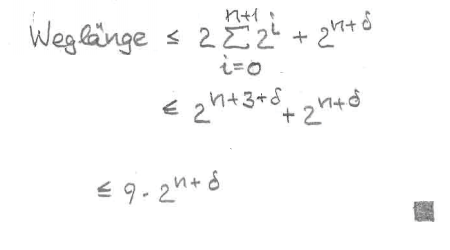
\includegraphics[width=0.3\textwidth]{9-kompetiv-beweis.png}
  \caption{Bsp. Kompetitivitätsbeweis}
\end{figure}


\end{document}